\documentclass[10pt,letterpaper]{article}

\usepackage[utf8]{inputenc}
\usepackage[spanish,es-nodecimaldot]{babel}
\usepackage{amsmath}
\usepackage{amssymb}
\usepackage{graphicx}
\usepackage{mathtools}

\usepackage{multicol}

\usepackage{enumitem}

\usepackage[top=1in, bottom=1in, left=1in, right=1in]{geometry}

\renewcommand{\arraystretch}{1.5}

\begin{document}

\begin{titlepage}
    \centering

    {\scshape\LARGE Universidad Nacional Autónoma de México \par}

    \vspace{1cm}
    {\scshape\Large Facultad de Ciencias\par}
    \vspace{1.5cm}

    \begin{center}
        
\includegraphics[scale=.1]{../../assets/img/logo.png}
    \end{center}

    \vspace{.8 cm}

    {\LARGE Tarea 05: \par}
    {\huge\bfseries Algoritmo genético simple y bloques constructores\par}

    \vspace{0.5cm}
    \large{\itshape{Pablo A. Trinidad Paz}} \small{ - 419004279}

    \vfill

    Trabajo presentado como parte del curso de
    \textbf{Cómputo Evolutivo}
    impartido por el profesor \textbf{Mario Iván Jaen Márquez}. \par
    \vspace{0.5cm}
    Fecha de entrega: \textbf{Jueves 28 de Marzo de 2019}.
\end{titlepage}

\begin{enumerate}
    \item Tenemos dos cromosomas padres distintos en un SGA con codificación binaria,
          cada uno con $L$ bits. Seleccionamos aleatoriamente un punto de cruza
          $c \in {1,...,L-1}$ y realizamos la cruza de un punto. ¿Cuál es la probabilidad
          de que ambas soluciones hijas sean clones (idénticas) de sus padres?\\[\baselineskip]
        \textbf{Solución:} Sean $a$ y $b$ los cromosomas padres tal que $a \neq b$ y $c$ es
        el punto de cruza descrito anteriormente, entonces los hijos $p$ y $q$ de la cruza
        de $a$ y $b$ resultan en
            \begin{equation*}\begin{split} \begin{aligned}
                p &= a_1 + b_2 \\
                q &= b_1 + a_2
            \end{aligned} \end{split} \end{equation*}
        donde $a_1$ y $b_1$ son las cadenas de los cromosomas padres $a$ y $b$
        respectivamente antes del punto de cruza $c$ y $a_2$ y $b_2$ son las cadenas después del
        punto de cruza. Para que $p$ y $q$ sean hijos idénticos a los padres se tiene que cumplir
        que $a_1 = b_1$ o $b_2 = a_2$, por lo tanto la probabilidad de que eso suceda dependerá
        del la posición del punto de cruza y la longitud de las sub-cadenas que genera. En otras
        palabras estamos buscando la probabilidad de que exista una sub-cadena $s$ de $a$ y $b$
        en los índices $[0, c]$ o $[c, L-1]$
    \item El problema \textit{\textbf{one-max}} consiste en buscar una cadena binaria de $L$
          bits con el mayor número de unos posible, es decir, el fitness de una cadena es el
          número de unos que contiene, por lo que se quiere maximizar $f(x) = \sum_{i=1}^{L} x_i$
          con $x_i \in \{0, 1\}$. Por supuesto que podemos resolver este problema de forma sencilla
          escribiendo $1$s consecutivamente en la solución, pero estamos interesados en ver si
          el SGA puede resolverlo. Implementa en Python el SGA usando
        \begin{itemize}
            \item Selección proporcional (FPS)
            \item Cruza de un punto con $P_c = 0.7$
            \item Mutación bit a bit con $P_m = 0.01$
            \item Tamaño del cromosoma $L= 30$
            \item Límite de generaciones: $100$
            \item Tamaño de población: $20$
        \end{itemize}
        \begin{enumerate}
            \item Lanza 20 simulaciones del algoritmo y grafica el fitness del mejor
                  individuo y el fitness de la población como función del número de
                  generación.
        \end{enumerate}
        \begin{multicols}{2}
            \begin{center}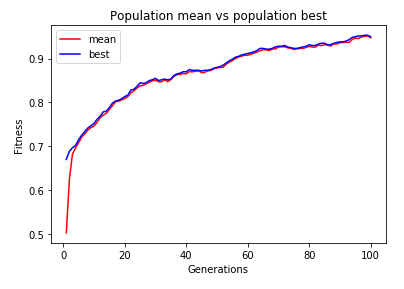
\includegraphics[scale=0.5]{./assets/ex2_mean.png}\end{center}
            \begin{center}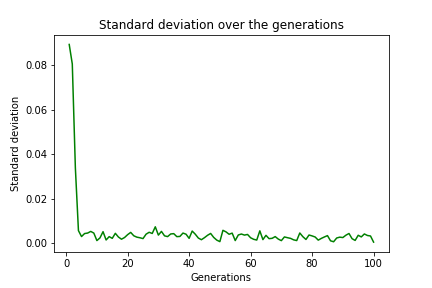
\includegraphics[scale=0.5]{./assets/ex2_std.png}\end{center}
        \end{multicols}
    \item Usando el paquete SCHEMATAX de Python: https://github.com/iSTB/python-schemata
          vamos a validar de forma experimental el teorema de los esquemas de J. Holland,
          calculando los esquemas procesados en cada iteración de SGA para observar los
          bloques constructores. \\
          Usando el problema anterior
        \begin{enumerate}
            \item Grafica el orden promedio y tamaño de definición promedio de
                  los esquemas procesados.
            \item Considerando que un esquema tiene bajo orden si está por debajo
                  del orden promedio y de igual forma tiene bajo tamaño de definición
                  si está por debajo del tamaño de definición promedio. Gracia el
                  orden promedio y tamaño de definición promedio de los bloques
                  constructores.
            \item Grafica el histograma de frecuencias sobre los bloques constructores
            \item Selecciona los 10 bloques constructores más frecuentes.
        \end{enumerate}
\end{enumerate}

\end{document}